\chapter{Exercise 3}
In this part we setup both shader uniformas and vertex attributes in both shader code and C++ code.
This is also an introduction to a very simple type of animation called vertex blending performed in
the vertex shader using GLSL.

\section{Part 1 and 2}
In the figure \ref{fig:exercise_3_part_1} we can see how vertex blending works in the program.

\begin{figure}[ht!]
	\begin{center}
		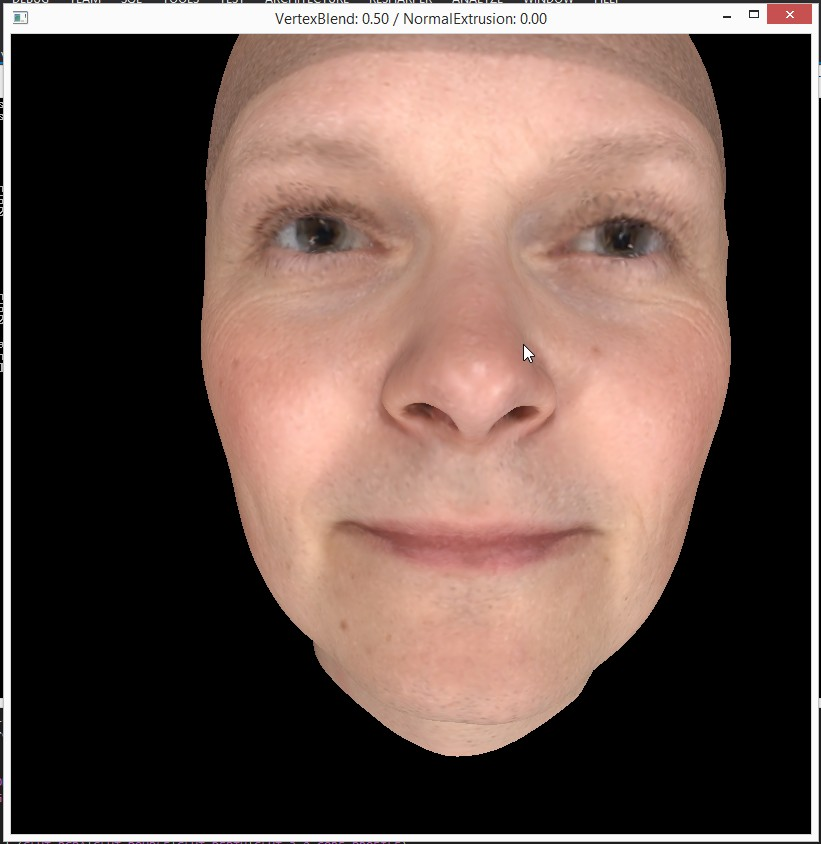
\includegraphics[width=0.5\textwidth]{figures/exercise_3_part_1}
	\end{center}
	\vspace{-4.5ex}\caption{Exercise 3 part 1 output}
	\label{fig:exercise_3_part_1} 
\end{figure}
I also modified the vertex shader to move the vertex along the normal direction by the amount specified
by normalExtrusion. This can be seen in the figure \ref{fig:exercise_3_part_2}.
\clearpage
\begin{figure}[ht!]
	\begin{center}
		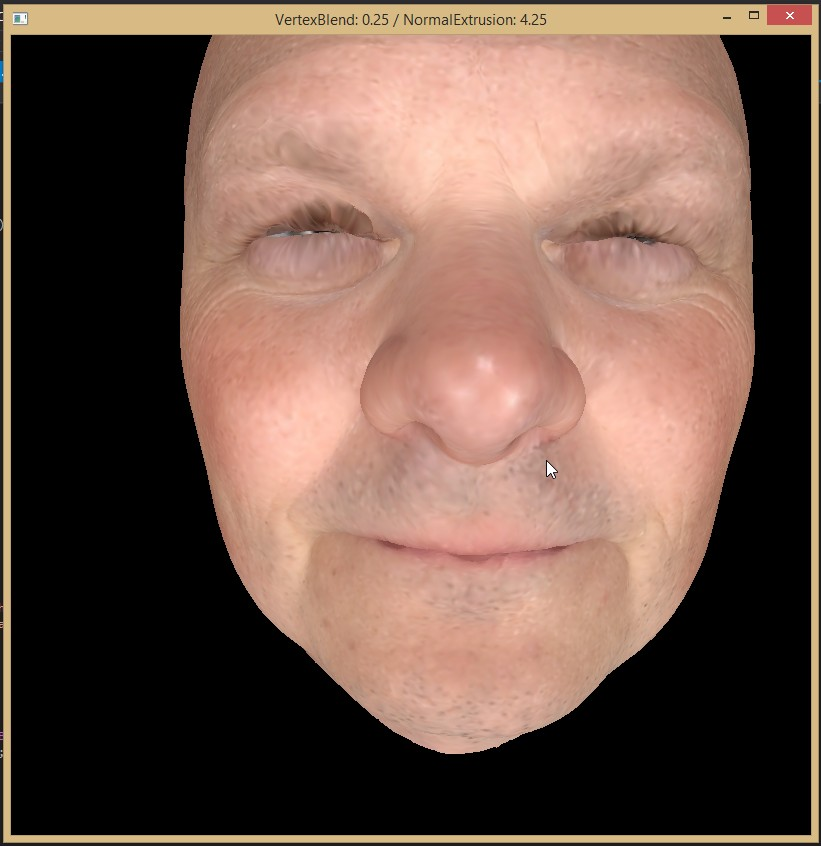
\includegraphics[width=0.5\textwidth]{figures/exercise_3_part_2}
	\end{center}
	\vspace{-4.5ex}\caption{Exercise 3 part 2 output}
	\label{fig:exercise_3_part_2} 
\end{figure}

All this transformations are done by the code in vertex shader:

\begin{lstlisting}[language=cpp, caption={Vertex blending}]
uniform mat4 projection;
uniform mat4 modelView;
uniform float blendValue;
uniform float normalExtrusion;

in vec3 position1;
in vec3 color1;
in vec3 position2;
in vec3 color2;
in vec3 normal1;
in vec3 normal2;

out vec3 colorV;
out vec3 position;

void main (void) {
	vec3 blendVector = vec3(blendValue);
    colorV = (1 - blendVector) * color1 + (blendVector * color2);
	vec3 normal = (1 - blendVector) * normal1 + (blendVector * normal2);
	position = (1 - blendVector) * position1 + (blendVector * position2) + (normal * normalExtrusion);
	gl_Position = projection * modelView * vec4(position, 1.0);
}
\end{lstlisting}
\clearpage

\section{Part 3}
\begin{description}
\item[Difference between a vertex attribute and a vertex uniform]
	Vertex attribute is a ,,vector'' of values, specified for each vertex, 
	while uniforms are sort of ,,constant'' values - the same value for all the vertices. 
	Both can be changed between the callbacks of a drawing function. 
\item[Vertex shader]
	The vertex shader manipulates the attributes of vertices, which are the corner points of displayed objects.
	It is a part of the early steps in the pipline where transforming of vertex location from one coordinate
	system to another is done. It computes the representation of a vertex in clip coordinates for the rasterizer.
\item[Fragment shader]
	The fragment shader takes care of how the pixels between the vertices look like (their color).
	Is is a part of rasterization step, where pixels between the vertices are coloured. 
\item[Between vertex shader and the fragment shader]
	Pixels are usually interpolated between the defined vertices in vertex shader following specific rules
	and passed through to the fragment shader.
\item[Blending the color in the fragment shader]
	It is possible and it is usually done there to obtain better quality. There is a special function for blending
	called mix, and it will be done per pixel not per vertex. However doing it in fragment shader can result in 
	lower performance.
\end{description}
\clearpage

\section{Part 3}
As it can be seen in the figure \ref{fig:exercise_3_part_3} I successfully obtained working 
discarding all pixels with even y coordinate using the code below.

\begin{lstlisting}[language=cpp, caption={Discarding pixels}]
in vec3 colorV;
in vec3 position;
out vec4 fragColor;

void main(void)
{
	if (mod(round(position.y),2) == 0) discard;
    fragColor = vec4(colorV, 1.0);
}
\end{lstlisting}

\begin{figure}[ht!]
	\begin{center}
		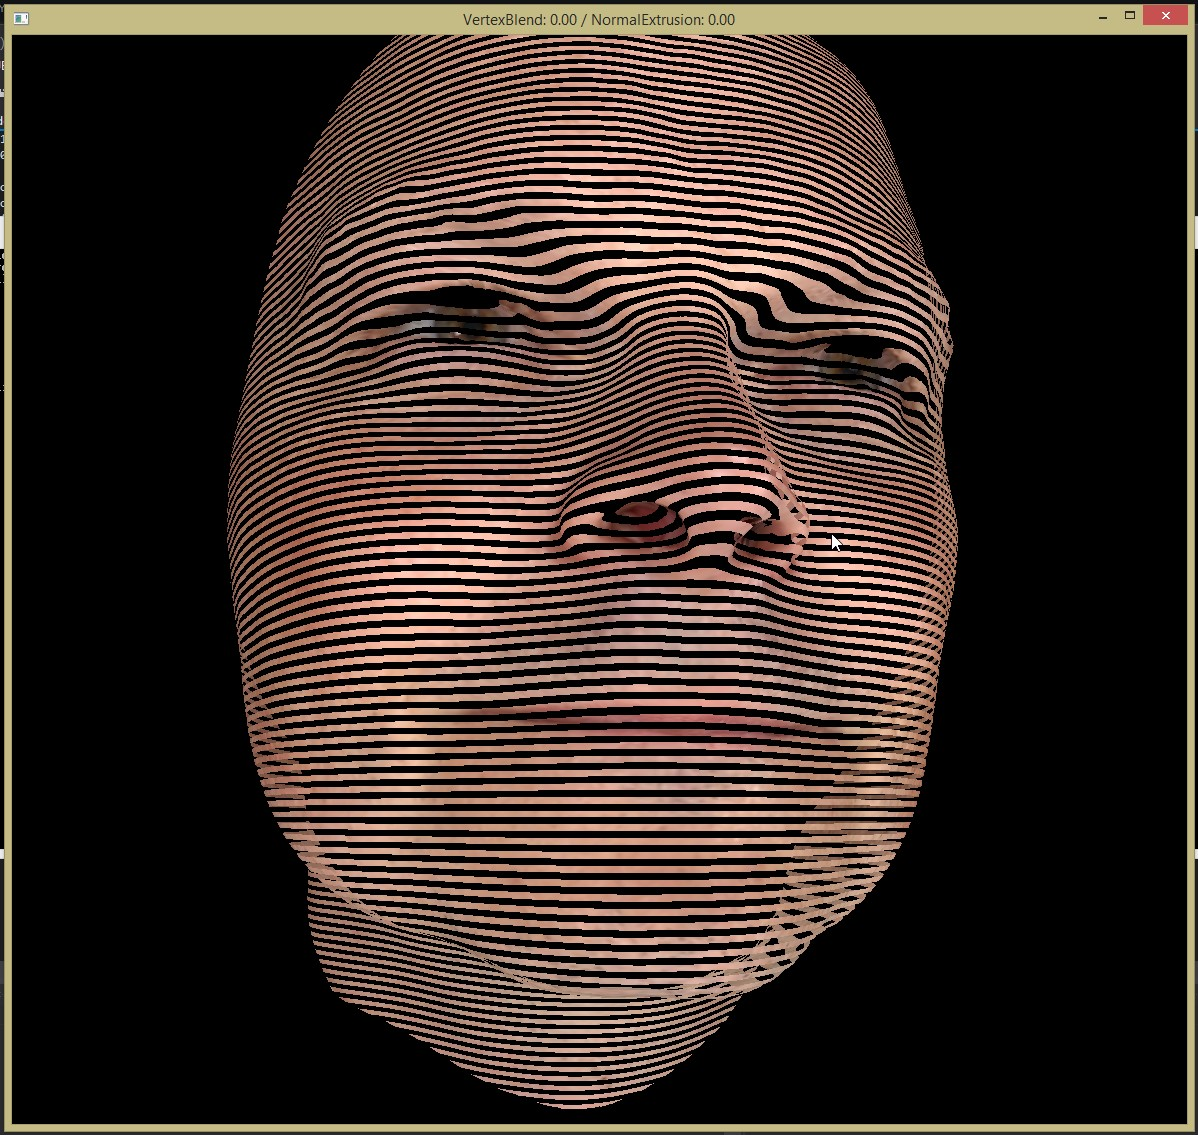
\includegraphics[width=0.9\textwidth]{figures/exercise_3_part_3}
	\end{center}
	\vspace{-4.5ex}\caption{Exercise 3 part 3 output}
	\label{fig:exercise_3_part_3} 
\end{figure}

